\documentclass[a4paper]{article}

\usepackage{amsmath}
\usepackage{amssymb}
\usepackage[margin=1.5cm,
            includefoot,
            footskip=30pt]{geometry}
\usepackage{layout}
\usepackage{graphicx}
\usepackage{subcaption}

\usepackage{biblatex}
\bibliography{main.bib}

\title{Recognising and evaluating the effectiveness
       of extortion in the Iterated Prisoner's Dilemma}
\author{Vincent A. Knight \and Nikoleta E. Glynatsi}
\date{\today}


\begin{document}

\maketitle

\begin{abstract}
    The Iterated Prisoner's Dilemma is a model for rational and evolutionary
    interactive behaviour. It has applications both in the study of human social
    behaviour as well as in biology.

    This game is used to understand when and how a rational individual might
    accept an immediate cost to their own utility for the direct benefit of
    another.

    Much attention has been given to a class of strategies for this game, called
    Zero Determinant strategies. It has been theoretically shown that these
    strategies can ``extort'' any player.

    In this work, an approach to identify if observed strategies are playing in
    a Zero Determinant way is described. Furthermore, experimental analysis of
    a large tournament with 204
    strategies is considered. In this setting
    the most highly performing strategies do not play in a Zero Determinant way.
    This suggests that whilst the theory of Zero Determinant strategies
    indicates that memory is not of fundamental importance to the evolution of
    cooperative behaviour, this is incomplete.
\end{abstract}

\section{Introduction}\label{sec:introduction}

% TODO Write short introduction and literature review.
% - Describe P&D,
% - Describe SP,
% - Describe Hilbe 2013 (evolution of extortion)
% - Describe Knight et al
% - statement about reproducibility of work

\section{Recognising Extortion}\label{sec:delta-zd-strategies}


In~\cite{Press2012}, given a match between 2 memory-one strategies, the
concept of Zeto-Determinant (ZD) strategies is introduced. The main result of
that paper showed that given two players \(p, q\in\mathbb{R}^2\) a linear
relationship between the players scores could be forced.

Assuming the utilities for player \(p\) are given by \(S_x=(R, S, T, P)\) and
for player \(q\) by \(S_y=(R, T, S, P)\) and that the stationary scores of each
player is given by \(S_X\) and \(S_Y\) respectively. The main result
of~\cite{Press2012} is that if

\begin{equation}\label{eqn:linear_relationship_for_p}
    \tilde p=\alpha S_x + \beta S_y + \gamma
\end{equation}

or

\begin{equation}\label{eqn:linear_relationship_for_q}
    \tilde q=\alpha S_x + \beta S_y + \gamma
\end{equation}

where \(\tilde p = (1 - p_1, 1 - p_2, p_3, p_4)\) and
\(\tilde q = (1 - q_1, 1 - q_2, q_3, q_4)\) then:

\begin{equation}
    \alpha S_X + \beta S_Y + \gamma = 0
\end{equation}

This work is interested with identifying a test for the reverse problem: given a
\(p\in\mathbb{R}^4\) how does one identify \(\alpha, \beta, \gamma\) if they
exist.

Note that equation~\ref{eqn:linear_relationship_for_p} can be expressed linear
algebraically as:

\begin{equation}\label{eqn:linear_algebraic_equation_for_p}
    Mx=\tilde p  \qquad x=(\alpha, \beta, \gamma)
\end{equation}

with \(M\in\mathbb{R}^{4\times 3}\) given by:

\begin{equation}\label{eqn:definition_of_M}
    M =
    \begin{bmatrix}
        R & R & 1\\
        S & T & 1\\
        T & S & 1\\
        P & P & 1
    \end{bmatrix}
\end{equation}

% TODO What is the rank of M? Can we prove something about it?

Note that in general, equation (\ref{eqn:linear_algebraic_equation_for_p}) will
not necessarily have a solution. From the Rouché-Capelli theorem~\cite{}% TODO
if there is a solution it is unique as \(\text{rank}(M)=3\) which the dimension of
the variable \(x\)). Furthermore, removing a single row of \(M\) would
ensure that the corresponding matrix is invertible. This corresponds to the fact
that a ZD strategy is defined by only 3 of its values.

As an example, consider the known ZD strategy \(p=(8 / 9, 1 / 2, 1 / 3, 0)\)
from~\cite{Stewart2012} which is referred to as \texttt{Extort-2}. In the
standard case of \((R, S, T, P)=(3, 0, 5, 1)\) the inverse
of \(M_{(4)}\) (removing the last row of \(M\)) is given by:

\begin{equation}\label{eqn:inverse_of_M4}
    M_{(4)}^{-1} =
    \left[\begin{matrix}1 & - \frac{3}{5} & - \frac{2}{5}\\1 & - \frac{2}{5} & - \frac{3}{5}\\-5 & 3 & 3\end{matrix}\right]
\end{equation}

This allows us to find the \(x=(\alpha, \beta, \gamma)\) corresponding to
\(\tilde p\):

\begin{equation}\label{eqn:alpha_beta_gamma_for_extort_2}
    x = M_{(4)}^{-1}\tilde p_{(4)} =
    \left[\begin{matrix}\frac{1}{18} & - \frac{1}{9} & \frac{1}{18}\end{matrix}\right]
\end{equation}

Using (\ref{eqn:linear_algebraic_equation_for_p}) gives that these values lead
to the correct value for \(p_4=0\) confirm that \(p_4\) is a ZD strategy.

This approach could in fact be used to confirm that a given strategy \(p\)
represents is ZD. However, in practice, if a closed form for \(p\) is not
known, then due to measurement and/or numerical error this would not work.

Thus, an approach based on least squares~\cite{Golub2013} is proposed. This
approach finds the best fitting \(\bar x=(\bar\alpha, \bar\beta,
\bar\gamma)\) which minimises:

\begin{equation}\label{eqn:r_squared}
    \text{SSError} = \|M x-\tilde p\|_2^2 = \sum_{i=1}^{4}\left((M\bar x)_i-\tilde p_i\right)^2
\end{equation}

Note that \(\text{SSError}\) which is the square of the Frobenius
norm~\cite{Golub2013} becomes a measure of how close \(p\) is to being a ZD
strategy.

In~\cite{Press2012} a particular type of ZD is defined, if:

\begin{equation}\label{eqn:constraint_for_extortion}
    P(\alpha + \beta)+\gamma=0
\end{equation}

then the player can ensure they get a score at \(\chi\) times
better than the opponent with. This extortion coefficient is given by:

\begin{equation}\label{eqn:definition_of_chi}
    \chi=\frac{-\beta}{\alpha}
\end{equation}

Thus, if (\ref{eqn:constraint_for_extortion}) holds and \(\chi >1\) a player is
said to extort their opponent. Recalling (\ref{eqn:definition_of_M}), equation
(\ref{eqn:constraint_for_extortion}) corresponds to the last row of \(M\), thus
a player \(p\) extorts their opponent if and only if \(p_4=0\) and the estimated
\(\chi > 1\). Using the method of least squares, the strategy \(p\) can be
considered ZD for a given threshold of \(\text{SSError}\) and \(\chi\) can be
approximated.  Figure~\ref{fig:examples_of_extortion} illustrates this for
potential strategies: for all of these we see that for the strategy to be
extortionate \(p_2\) and \(p_3\) seem to have a linear relationship.

\begin{figure}[!htbp]
    \begin{center}
        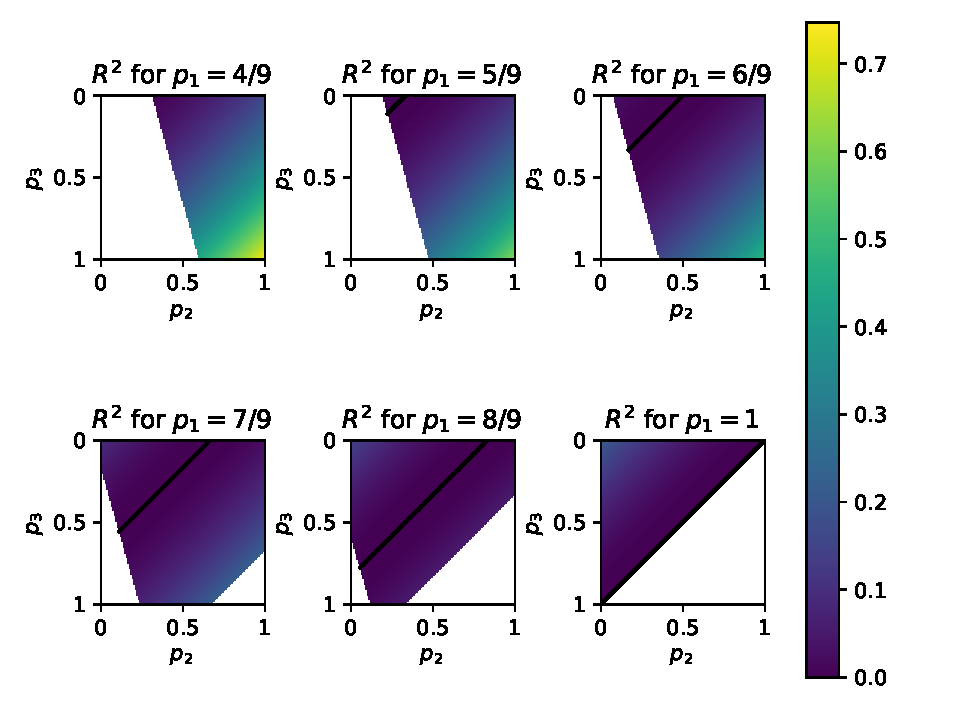
\includegraphics[width=\textwidth]{assets/img/examples_of_extortion/main.pdf}
        \caption{Strategies of the form:
                 \(p=(p_1, p_2, p_3, 0)\). The solid line shows the values for
                 which \(\text{SSError} < 10 ^ {-6}\). Only values for which \(\chi > 1\) are
                 displayed, strategies outside of this region can never be
                 extortionate.}
        \label{fig:examples_of_extortion}
    \end{center}
\end{figure}

By observing interactions (human or otherwise), the transition rates of given
individuals can be approximated and this approach can be used to recognise
extortionate behaviour. Note that if the environment is noisy then no strategy
can be considered to be extortionate.
% TODO Add reference and possibly move
% this I. The reason for it, is that we cannot have $P(C|CC)=0$ in a noisy
% environment.

% TODO Add discussion about missing observations.
% Technically if a strategy has missing observations then it is definitely ZD.

In the next section, this idea will be illustrated by observing the interactions
that take place in a computer based tournament of the IPD\@.

\section{Numerical experiments}\label{sec:numerical-experiments}

In~\cite{Stewart2012} results from a tournament with
19 strategies,
was presented with specific consideration given to ZD strategies. This
tournament is reproduced here using the Axelrod-Python
project~\cite{Knight2016}. To obtain a good measure of the corresponding
transition rates for each strategy all matches have been run for
2000 turns and every match has been
repeated 60 times.
% TODO Archive data.

Using the pair wise interactions the transition rates \(p,
q\) can be measured and the steady state probabilities inferred and compared to
the actual probabilities of each state.
This is done numerically by computing the singular eigenvector of the
matrix: \(A\) \cite{Stewart2009}:

\[
    A =
    \begin{bmatrix}
        p_1 q_1 & p_1 (1 - q_1) & (1 - p_1) q_1 & (1 -p_1) (1 - q_1) \\
        p_2 q_2 & p_2 (1 - q_2) & (1 - p_2) q_2 & (1 -p_2) (1 - q_2) \\
        p_3 q_3 & p_3 (1 - q_3) & (1 - p_3) q_3 & (1 -p_3) (1 - q_3) \\
        p_4 q_4 & p_4 (1 - q_4) & (1 - p_4) q_4 & (1 -p_4) (1 - q_4) \\
    \end{bmatrix}
\]

Figure~\ref{fig:computed_probabilities_vs_theoretic_probabilities}
shows a regression line fitted to every pairwise interaction with a reported
\(R^2\) value (pairwise interactions with missing states were omitted). This
serves to validate the approach: a part from some edge cases the relationship is
consistent.

\begin{figure}[!htbp]
    \centering
    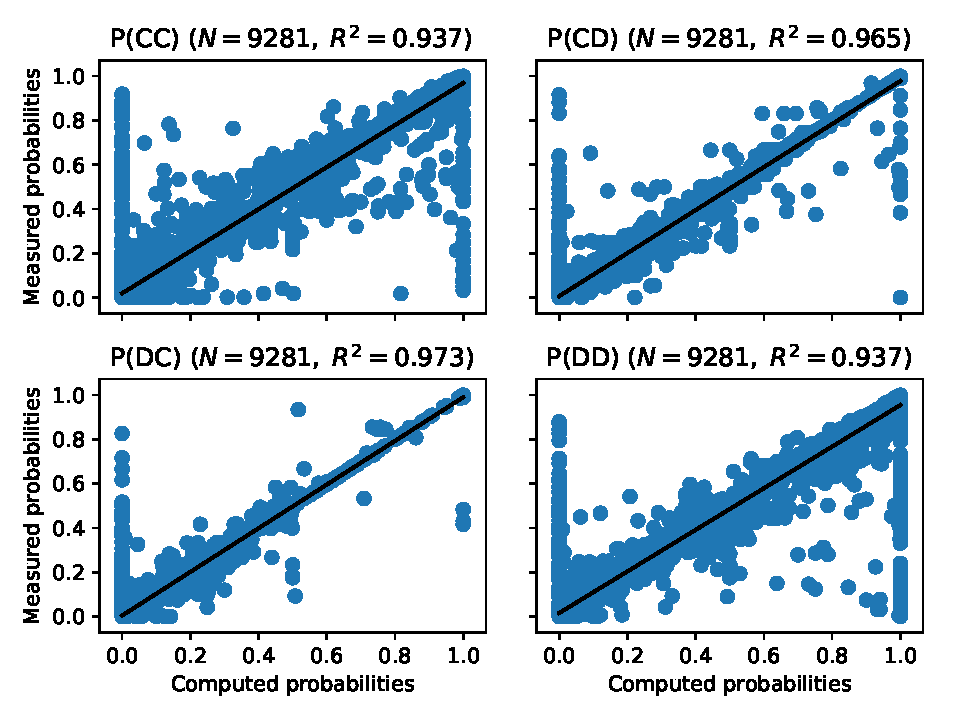
\includegraphics[width=.8\textwidth]{./assets/img/computed_probabilities_vs_theoretic_probabilities/main.pdf}
    \caption{The
        relationship between the steady state probabilities inferred from the
        measured transitions and the actual steady state probabilities. A linear
        regression line is included validating the approach.}
    \label{fig:computed_probabilities_vs_theoretic_probabilities}
\end{figure}

Figure~\ref{fig:SSError_overall_in_stewart_plotkin} shows the \(\text{SSError}\)
values for all the strategies in the tournament, as reported
in~\cite{Stewart2012} the extortionate strategy (which has an expected
\(\text{SSError}\) approximately 0) gains a large number of wins.
Whilst~\cite{Stewart2012} described the performance of each strategy, this
approach also informs the behaviour of a strategy when their opponent is not a
memory one strategy thus not creating a Markov chain.

\begin{figure}[!htbp]
    \centering
    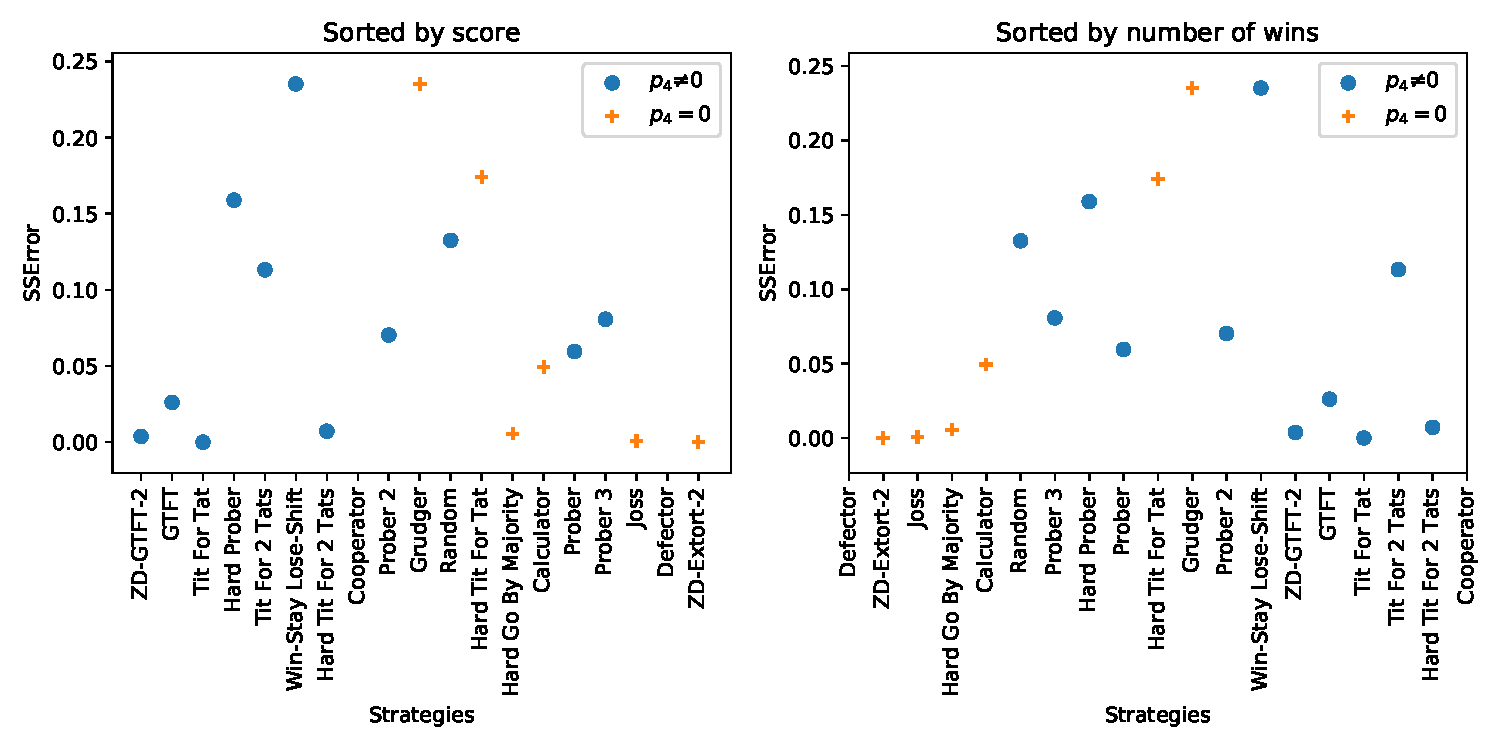
\includegraphics[width=.8\textwidth]{./assets/img/SSError_overall_in_stewart_plotkin/main.pdf}
    \caption{\(\text{SSError}\) for the strategies of~\cite{Stewart2012}, ordered both by
    number of wins and overall score. Cooperator and Defector are omitted as
    they do not visit all the states.}
    \label{fig:SSError_overall_in_stewart_plotkin}
\end{figure}

Here, the work of~\cite{Stewart2012} is extended by investigating a tournament
with 204
strategies.

The results of this analysis are shown in
Figure~\ref{fig:SSError_and_probabilities_in_full}. The top ranking strategies
by number of wins seem to be extortionate (but not against all strategies) and
it can be seen that a small sub group of strategies achieve mutual defection.
The top ranking strategies according to score all achieve mutual cooperation and
do not extort each other, however they
\textbf{do} extort a number of the lower ranking strategies.

\begin{figure}[!htbp]
    \centering
    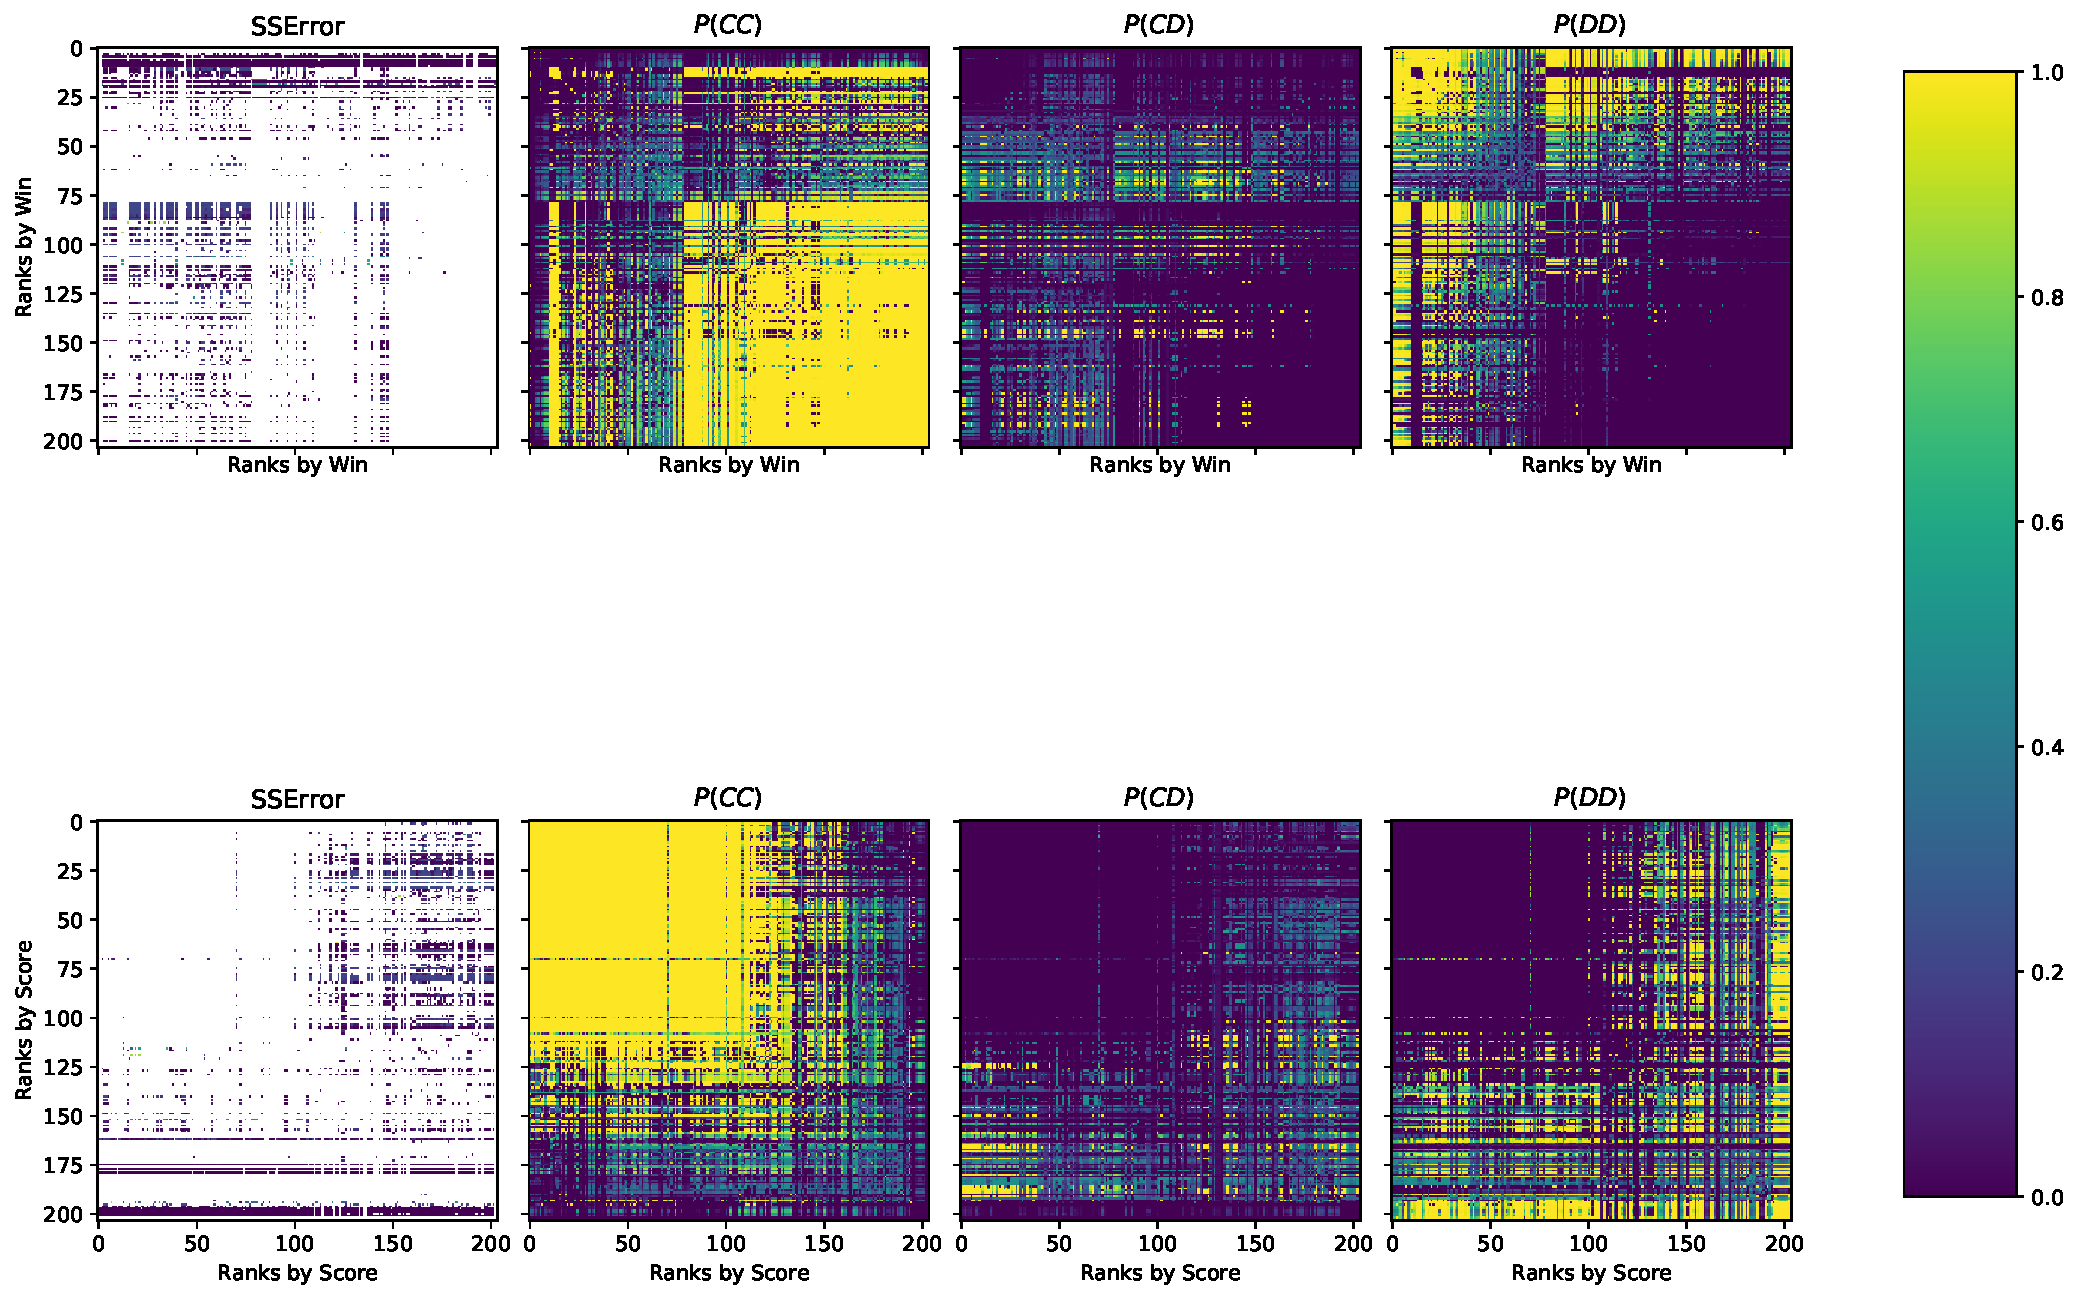
\includegraphics[width=.8\textwidth]{./assets/img/SSError_and_probabilities_in_full/main.pdf}
    \caption{\(\text{SSError}\) for the strategies for the full tournament. Only
    strategy interactions for which \(p_4=0\) and \(\chi>1\) are displayed.}
    \label{fig:SSError_and_probabilities_in_full}
\end{figure}


\section{Conclusion}\label{sec:conclusion}

This work defines an approach to measure whether or not a player is playing a
strategy that corresponds to an extortionate strategy as defined
in~\cite{Press2012}. Indeed Figure~\ref{fig:examples_of_extortion} classifies
all extortionate strategies. This is done through a linear algebraic approach
for approximating the solution of a linear system. Using this, a very large
number of pairwise interactions is simulated and in fact very few strategies are
found to act extortionately.

The work of~\cite{Press2012}, whilst showing that a clever approach to taking
advantage of another memory one strategy exists: this is incomplete. Whilst the
elegance of this result is very attractive, just as the simplicity of the
victory of Tit For Tat in Axelrod's original tournaments was, it is incomplete.
Whilst extortionate strategies achieve a high number of wins they do not
achieve a high score which corresponds to the fitness landscape in an
evolutionary sense. This confirms
the findings of~\cite{Moran1707} in which sophisticated strategies resist
evolutionary invasion of shorter memory strategies.

This work can be used to classify plays of the IPD\@: data can be collected from
actual interactions (in lab or in the field). Furthermore, this allows for a
classification method similar to the notion of fingerprinting presented
in~\cite{Ashlock2008}. Trained strategies can potentially be classified as
extortionate or not or it could be possible to even constraint the reinforcement
learning approaches that are becoming prevalent in the literature.

\printbibliography

\end{document}
